\section{Product perspective}
\subsection{Scenarios}

\begin{enumerate}
      \item \textbf{Student's first platform access}\\
      Alessandro Sesenna is a Computer Science student who wants to register with the S\&C platform to start looking for internship projects. After entering the URL in the web Browser (such as Mozilla Firefox, Internet Explorer, etc.) the user needs to authenticate through the university's Single Sign On system. When the authentication process ends, the system recognizes that this is his first access and redirects him to an initial page. 
      Here, Alessandro is asked to decide among different options about his favorite academic interests. The system has already selected a list of possible fields of interest, based on Alessandro's course of study, which the platform received upon the first registration. Among the options he selects "Data Science", "SQL programming" and "DataBase management". Once this is done, the system creates an ad-hoc homepage containing the various offers, previously posted by companies, ordered by suitability with his chosen interests. Alessandro won't be able to send a contact request to the companies shown in the homepage until he has completed the "My CV" procedure.

      \item \textbf{Student inserts his CV information in the InitialForm}\\
      Federico Ferri is a student who is attending a university and has already registered with the S\&C platform.
      Federico wants to find an internship, so he logs into the system and is initially shown his personalized homepage. He starts scrolling through the various opportunities and notices an offer that is interesting to him. When he clicks on the contact button, the systems shows a pop-up, in which it is written that to communicate with a company is mandatory to first insert his information in the section "My CV".
      Federico clicks the button on the popup which redirects him to the "My CV" section. 
      This opens a form which will require the user to fill the following fields:
      \begin{enumerate}
		    \item Personal information (Name field, Contact information, Personal ambitions, etc.) 
		      \item Education (Academic background and Achievements)
                \item Work Experience (Job Title, Company Name, Duration, Technologies used, etc.)
            \item Technical and soft skills 
            \item Project and Research (Projects/Research title, Duration, Description, etc.)
            \item Extracurricular activities (Activity name, Organization/ Event, Achievements, etc.)
            \item Certification and training (Certification Name, Provider, Validity, etc.)
            \item Languages (Language, proficiency level, certification, etc.)
            \item Internship availability (here the student indicates whether he's willing to do an unpaid internship)
            \item Additional Information (Interests, reference contacts, etc.)
    \end{enumerate}
After filling all the fields the system will show a message confirming the success of the operation. 
     
      \item \textbf{Student search through the internships and contact the company}\\
     Nicolò Bilzi is a computer engineering student and is looking for a company specialized in data analysis to do his first summer internship. After registering at S\&C, choosing his favorite fields (big data, data science and data engineering) and filling the information in the ‘My CV’ section, Nicolò opens his homepage.
     On the homepage he can see several internship possibilities, and in particular Nicolò decides to click on the contact button next to the "Azure" company offer, which explains they are looking for a data engineer position to do a data manipulation project. After clicking the contact button the site automatically generates a personalized CV for the company that posted the advertisement and lets Nicoló revise it before sending it. If Nicoló approves the document, he will proceed to send it. Once the company sees his CV, and considers it valid, the two parties can agree on next steps. Instead, if the company doesn't consider the CV valid, they can discard the profile of Nicoló by clicking on the "discard" button.
      
      \item \textbf{A company publishes an advertisement about the internships they are offering}\\
    Alex Zurlini is an employee of "AudioServizi" company, which is looking for an electronic engineer to assign a project about headphones battery durability.
    His company has been already registered in the S\&C platform, so he logs in using his business credentials.
    Alex logs into the system and the personalized homepage with a list of potential students for their internship is shown.
    At the left upper corner, the user is able to open a sidebar, where, among the many choices, decides to click on the "Create Job Opportunity" button. 
    This screen bring Alex to a form, which includes the following fields:
    \begin{enumerate}
      \item Title 
      \item Job description (where he is assisted by the system, which utilizes AI to suggest an appropriate job description)
      \item Requirement (e.g. computer science degree, economics degree, etc.)
      \item Internship Duration (e.g. six months, one year, etc.)
      \item Internship availability (two options where the employee selects if the internship is paid)
      \item Other useful information (free text area)
    \end{enumerate}    

    Since they are looking for a figure to work on small battery research, puts in the \textit{"Title"} field \textit{"Electronics engineer"} and, below, in the \textit{"Job Description"} field, assisted by the platform, puts \textit{"Searching for an electronic engineer to commit to our research project on the durability of headphone batteries"}.
    A bachelor's degree in electronic engineering is required, so he selects it from the checkbox list that appears after clicking the \textit{"Requirement"} field.
    After selecting the duration of the position, the pay of the internship and adding additional useful information, he publishes the position by clicking on the \textit{"Publish"} button below the form. Once this is done, students that have registered on the system and meet the requirements in electronics engineering and indicated their interest in this subject will receive a notification of the available internship.
    
    
      \item \textbf{A student receive a notification about the availability of an internship that might interest her}\\
       Paola Rossi is a university student and when she registered to S\&C, among other preferences, she selected "robotics". A company called "Robotics S.P.A." posts the availability of an internship regarding the usage of robots in a medical environment on the platform. Since Paola selected "robotics" as a preference she receives a notification on her email. Since she's interested she clicks on the link at the end of the email and is redirected to the company's offer page. After reading all the information, she decides to contact the company.
       Since Paola has already completed her "My CV" section, she will be able to decide whether to contact the company by clicking on the contact button or simply be redirected to their homepage. The first option creates a personalized CV, shows it to Paola for reivew and, if everything is fine, send it to the company. 
      
      
      \item \textbf{A company receives a notification about the availability of a student CV corresponding to their needs}\\
      Giuseppe Latino is an HR representative for “Computerz SPA” and is subscribed to S\&C, where his company has opened an internship position. Francesco Damante is a computer science student who has just subscribed to the platform and completed his "My CV" section. He has characteristics that perfectly correspond to what Giuseppe’s company were searching for. Giuseppe receives an email notification, that recommends Francesco's profile for the internship they are offering. Once he opens it by clicking on the "View profile" button the system brings him to Francesco’s presentation page. To contact him Giuseppe clicks on the button next to Francesco’s name and a chat interface comes up. From this page he can start to exchange messages with him and arrange a meeting to do interviews and see if he fits the company’s requirements.
      
      \item \textbf{Student gives final feedback about the internship}\\
      Roberta Maniero has just finished her internship at the company "Dassault Systemes" and would like to leave a review of her experience. She opens the S\&C website and after logging in, opens the sidebar and selects the ‘Report’ button.
      The system automatically recognizes that the internship has ended and shows her a form to fill out entitled "Give us your final feedback". Here, Roberta writes down everything she liked, what she learned and what she would improve about her experience. To submit feedback, Roberta presses the "Submit" button.


      \item \textbf{The University receives the request to end an internship from a student and contacts the company to end it}\\
      Isacco Robuschi works as an employee at Politecnico Di Milano. He receives an email that informs him about a new complaint by one of the university's students. He clicks on the "See complaint" button. This opens a page that shows what the student has complained about. After reading the complaint which includes a request to end the internship, he clicks on the student name in the upper part of the page. This opens the student's profile for him where he finds the company contacts above the student name in his homepage. After discussing with the company the reasons behind this situation, they agree to end the internship. To do so, Isacco needs to open the student homepage and click on the "Terminate Internship" button. The platform will then ask him if he really wants to continue this process, to which he'll clicks the "Yes" button that will end the internship between the student and the company.      

      \item \textbf{Student complains with the university on the "Report Area" about his ongoing internship}\\
      Francesco Castellante is a Mechanic Engineering student and is conducting an internship with "Pipes S.P.A" which is a company that builds and sells pipes all around the world. Once Francesco signs in with S\&C, he selected as a preference "mechanics" and "3D design" hoping to find an internship that will help him optimize his skills in that field. Unfortunately, the company who accepted him is in a difficult period and all the employee are occupied so they aren't able to offer him the support needed. Instead of guiding him through the work, they told him to watch tutorials about how to use the technologies he has to employ to do the project they assigned to him. The problem is that the tutorials aren't as efficient as someone, who knows how the technology work explaining the basic functionalities and why things need to be done in a specific way. Since Francesco is a hard worker and wants this internship to be as educational as possible, he would like to file a complaint, hoping to prompt the company to assign him an employee that teaches him how to do this type of job. To do so, the platform offers two different sections, viewable after opening the toolbar, called "Report Area", where he can communicate with the university, and "Chat", where he can write to the employee responsible for his internship. Since he has already tried to speak with the HR manager of the company, and nothing changed, he decided to report it through the "Report Area" section. After writing his complaint and sending it, he needs to wait for an answer from the university.
      
      \item \textbf{The company complains about the student taking the internship}\\
      Marco Carta is a manager at the company ‘QS Informatics’ and supervises the work of Mirko Soragna, a computer engineering student, participating at their internship project as an aspirant data scientist. However, after following Mirko's work for two weeks, Marco realises that Mirko's programming skills aren't sufficient to do the job they assigned him. Marco therefore wants to contact Mirko's university to inform them that "QS Informatics" intend to terminate the internship. Marco, after logging into the S\&C platform, opens the sidebar and clicks on the ‘Report Area’ button. Here the site shows him the complete list of students who are doing an internship at his company. Marco then clicks on the name of ‘Mirko Soragna’, and is directed to his profile's page. Here Marco clicks on the "Report" button. This brings him to a page where he can insert the report on Mirko's work and describe all the details regarding his request to terminate the collaboration. After sending it, the site will send a notification to the university which will contact the student and inform him of the termination.
      
\end{enumerate}

\subsection{Domain class diagram}
\begin{figure}[H]
        \centering
        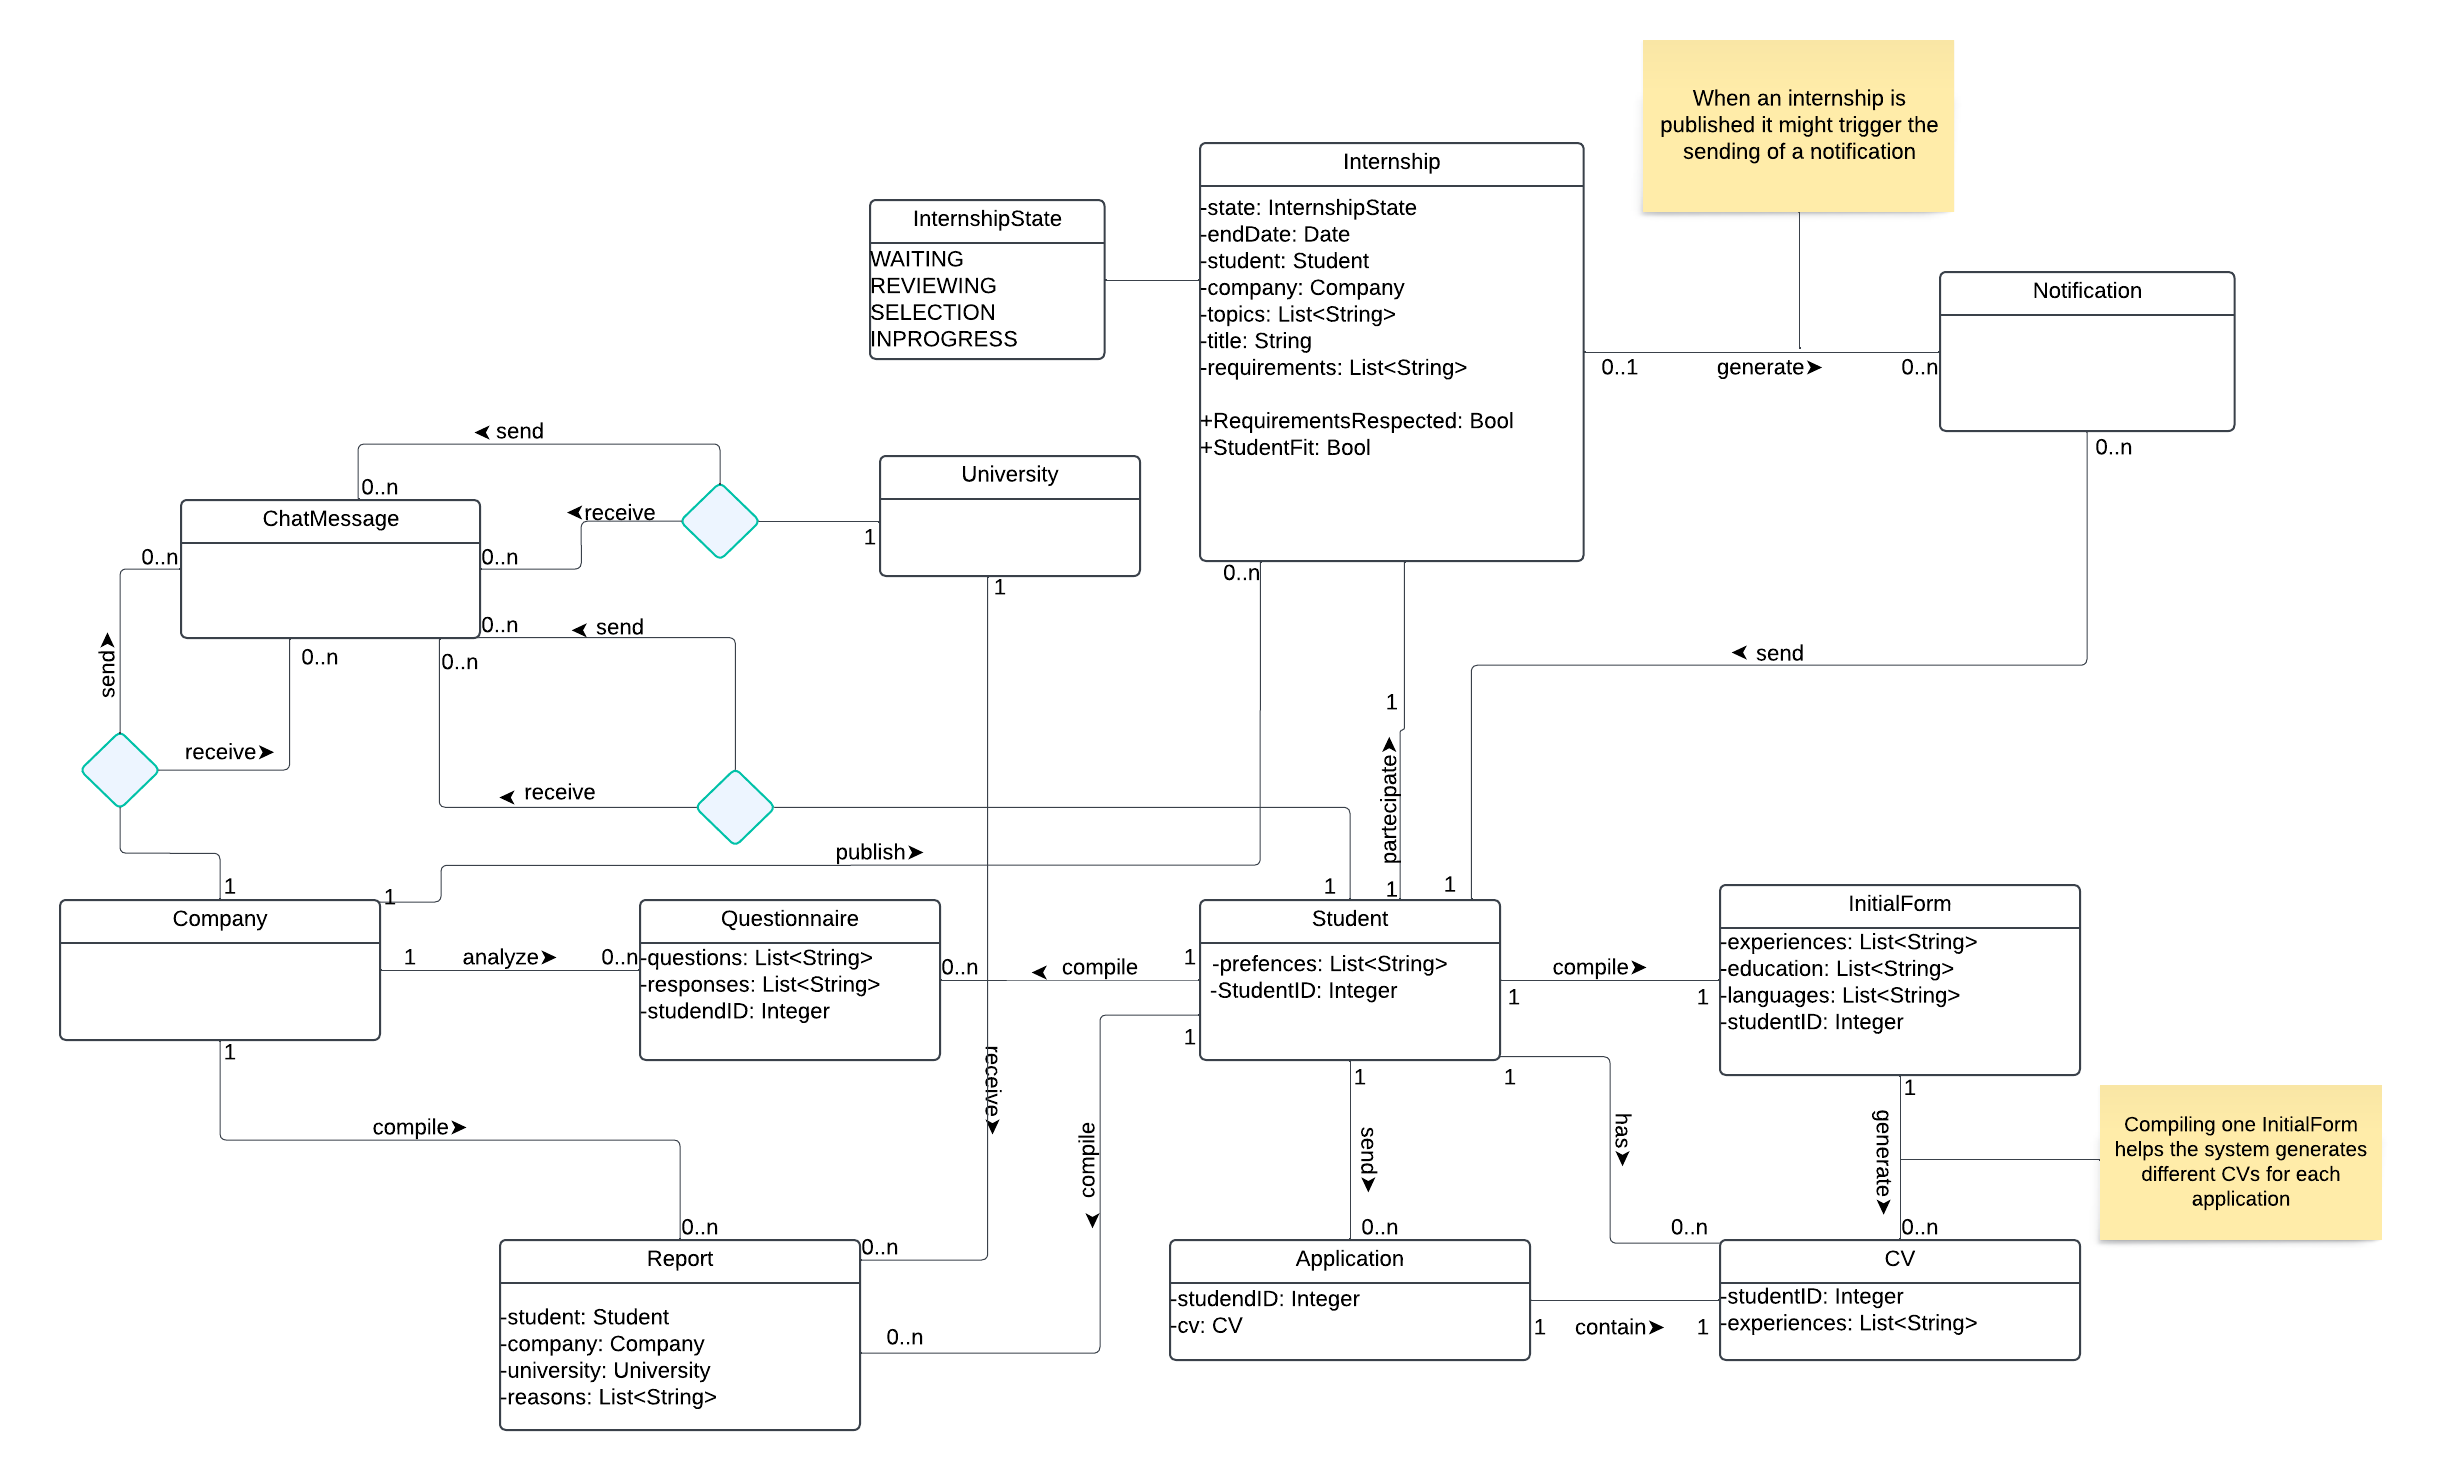
\includegraphics[width=0.8\textwidth]{RASD/Assets/ClassDiagram/Classdiagram.png}
        \caption{Class Diagram.}
        \label{fig:Class Diagram.}
    \end{figure}

\subsection{State diagrams}
The following discusses how the state of internships and complaints evolves in time, in order to have a better understanding of their lifecycle in the model.\\
\textbf{Internship}\\
When an internship is created by a company, it starts in a Waiting state. During this phase, students can: receive a notification about the publication of the internship, see it in their personalized homepage or can be contacted directly by the company. From the Waiting state there are two different ways of progressing. If the company contacted the student, this means that the internship enters directly the Selection state. Instead if it is the student who contacted them, it enters the Reviewing state. Here the company makes sure that the requirements listed in the published internship are respected by reading the student's CV and looking at his profile. If the answer to the check is negative, it goes back to the Waiting State. Instead, if the check is positive, the selection state is reached. Here it starts in a Contacting state where the company and the student through the platform chat section arrange a date for the interview. Once they come to an agreement, the meeting will be posted along with the link for the virtual room in the calendar of both of the parties. During this phase the student will also be asked to answer a questionnaire. Once the date for the interview comes the selection process reaches the Interviewing state. After the interview is finished, it will reach the Evaluating state where the company determines if the student is fit for the project. If he/she's fit, the internship will start and reach the InProgress state. Instead, if it doesn't, the internship will return to the waiting state. In the InProgress state it is explained with the use of substates that from a working phase if the company/student complains, the internship enters a Complaining state. From here the flow can either go back to the Working State or directly to the Terminated state if the complaint contains a termination request. From the Working state once the internship reaches its end, it will reach the Terminated state.\\
\begin{figure}[H]
        \centering
        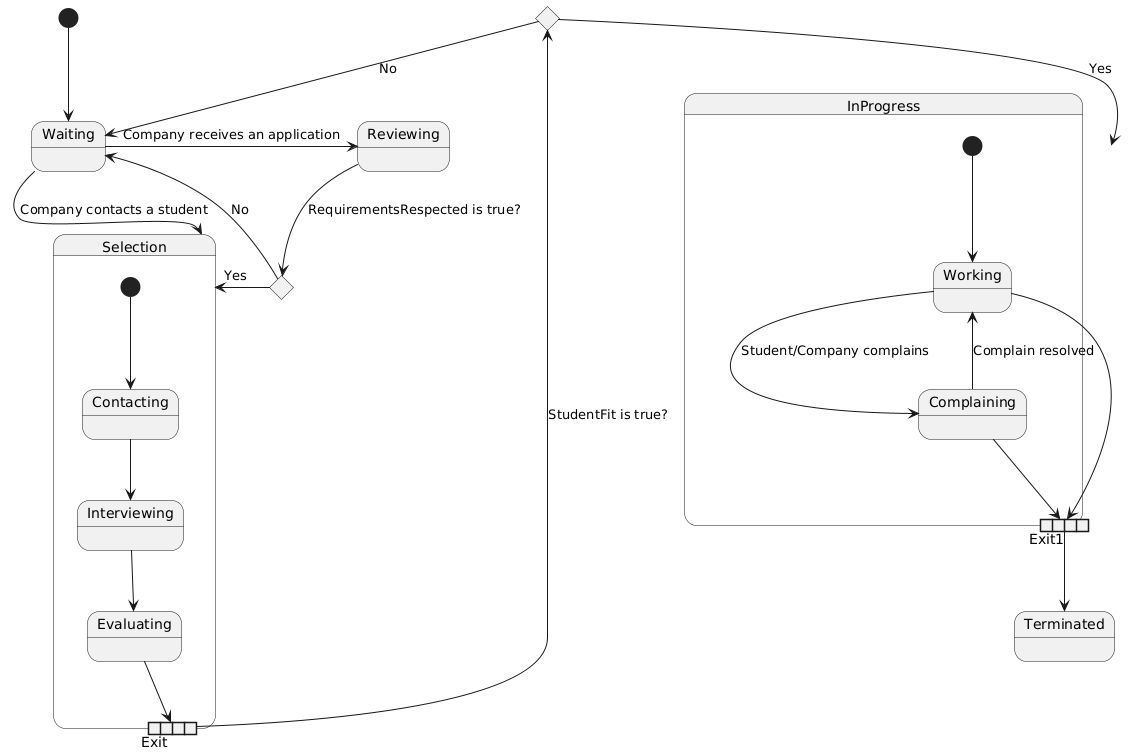
\includegraphics[width=0.8\textwidth]{Assets/Statecharts/Internship_SC.png}
        \caption{Internship state diagram.}
        \label{fig:Internship state diagram.}
    \end{figure}
\textbf{Complaint}\\
There are two ways of complaining, one is by opening the chat section which will permit the student and the company to communicate and resolve minor issues without involving the university. And the other one is by opening the Report Area which is a page where one of the two parties can directly communicate with the university. In this state chart, we'll analyze the processes of the second option.
When a user goes to the "Report Area" section it starts the complaint process which begins from a Sending state in which the user can write all the reasons of his complaint. Once the text is well written and complete the user can send it. Once it is sent, it goes to the Reading state where the complaint sent can be read. If it is a termination request, the university, which manages the interruption of the internships, will contact both parties and let them know the collaboration is ended, represented by the Terminated state. Instead, if it is a solvable situation, from the Reading state it will move to the Resolving state where the parties will start to communicate and try to come up with a solution. If the problem is addressed, the complaint will reach the Solved state and the internship can continue (in the internship statechart it will go back to the Working state), instead if a solution isn't found, the internship will terminate and the complain will reach the Terminated state.\\
\begin{figure}[H]
        \centering
        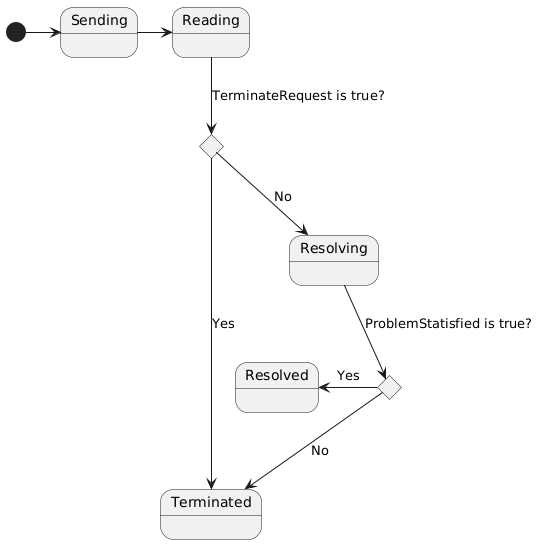
\includegraphics[width=0.8\textwidth]{Assets/Statecharts/Complain_SC.png}
        \caption{Complaint state diagram.}
        \label{fig:Complaint state diagram.}
    \end{figure}
\section{Product Functions}
\subsection{Reccomendation}
The Recommendation Function is a core feature of the S\&C platform that facilitates the matching process between students and companies by suggesting the most suitable opportunities based on the characteristics and preferences of both parties. 
For students the system analyzes their profiles, including their CV, skills, education, work experience, and preferences (e.g., type of internship, location, industry). Based on this data, it creates a personalized homepage where the upper internships showed are the ones that align closely with the student's qualifications and interests.
Instead, for companies, the system evaluates the requirements specified in their internship offer, such as required skills, educational background, and job type. It then recommends students whose profiles best meet these criteria, providing companies with a personalized homepage of potential candidates.
The recommendation process uses automated algorithms based on statistical analysis, keyword matching and possibly machine learning to identify relevant matches. Whenever a new student registers to the platform, insert his CV's information and is appetizing for a company, the system will send a notification to the company. The same happens when a company registers and posts an internship offer that might interest a student based on his topic preferences, in this case the system will send a notification to the student and update his homepage. The Recommendation Function ensures that students are connected with internships that suit their career goals while helping companies find candidates who match their needs, creating an efficient and effective matchmaking system.
\begin{figure}[H]
        \centering
        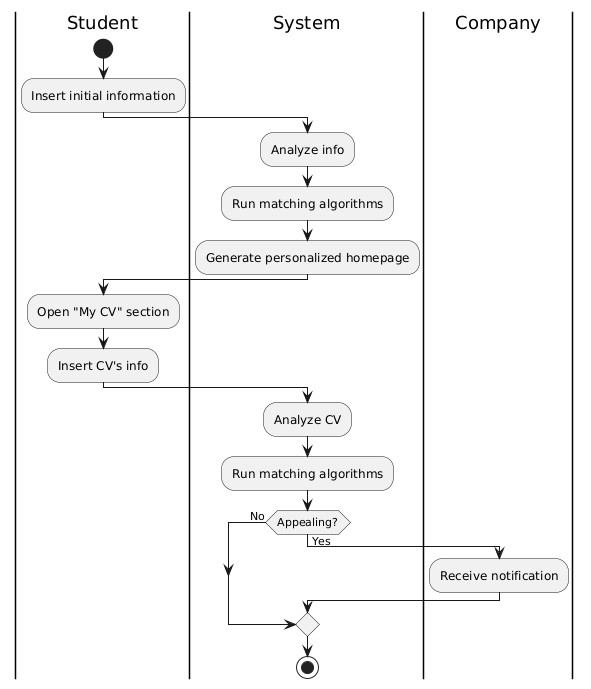
\includegraphics[width=0.8\textwidth]{RASD/Assets/ActivityDiagram/Reccomandation_AD2.png}
        \caption{Reccomandation activity diagram.}
        \label{fig:Reccomandation activity diagram.}
    \end{figure}
\subsection{Selection}
The Selection Function is used by companies and manages the steps through which companies evaluate and decide which students are fit to take parts to their internship programs. With this function the platform facilitates the evaluation, interview scheduling, and final selection of candidates in an efficient and organized manner. Is used by companies which firstly review and evaluate students applications. Once they select the student that is fit for their project, they can start by contacting them and, through the platform functionalities, start to arrange meeting interviews. 
The selection process follows these steps;
1.	Contacting: where companies evaluate and contact the student who sends them an application or directly contact a student that caught their attention in their personalized homepage.
2.	Interviewing: once they select a student they send them a questionnaire and an interview request to see if the student can be a good fit for their project. 
3. Evaluating: After the interview process, if the student is fit, through the contact page offered by the platform, they can submit a formal request to start the internship with the selected student.
\begin{figure}[H]
        \centering
        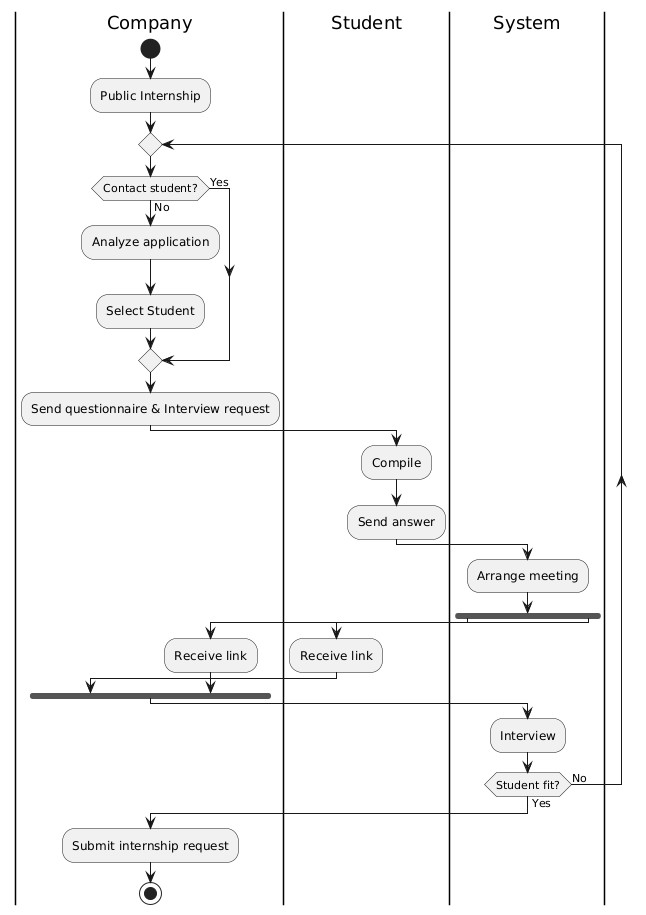
\includegraphics[width=0.8\textwidth]{RASD/Assets/ActivityDiagram/Selection_AD2.png}
        \caption{Selection activity diagram.}
        \label{fig:Selection activity diagram.}
    \end{figure}
\section{User charateristics}
\subsection{Student}
The student is a client who is able to access the S\&C platform through the SSO login. They use the platform with the goal of finding an interesting internship project to work on and learn new technologies used in a work environment. Their participation goes through several stages: first they sign into the platform, then they compile a form which asks them various information that will help S\&C to create their CVs. So every time a student wants to contact a company, the system will create a personalized CV tailored for the company needs. Each student receives also a notification every time a company posts an announcement on the platform, where the requirements fit the ones described by the student in his CV.
\subsection{Company}
The company is a client which represents a business entity that uses the S\&C platform to connect with students that might join their internship project programs. Companies use the platform to contribute to the students growth by offering them a real work experience. Their involvement takes place in several stages: it begins by creating a job opportunity, where they provide the title, a quick description of the internship they are offering, requirements and duration of the internships. They can manage the entire recruitment process through the platform. They can provide feedback on the student’s performance during the internship or at the end of it but, more importantly, they can propose changes to the system to improve the recruitment efficiency. They can also make complaints about the student’s work and ask for the termination of the internship or, more likely, contact the university to ensure that the issues that arise during the internship are addressed effectively. Each company receive a notification every time a student with the correct attributes for their project registers to the platform. The involvement of the companies helps strengthen the connection between schools and the workplace.
\subsection{University}
The university is a client that monitors and supports students during their internship. Its role is to ensure that student's learning experiences align with their educational goals and that internships meet the required standards. But also that their students are doing their job in a meticulous way by being notified from the companies when something doesn’t add up. Their involvement consists in  monitoring each student's progress during the internship and ensure that the experience provides meaningful learning opportunities. They are also responsible for handling complaints or issues that may arise during the internship, including resolving cases that require the internship to be interrupted.
\section{Assumptions dependencies and constrains}
The following domain assumptions must hold in the world:
\begin{enumerate}[label=\textbf{D\arabic*}:,ref=D\arabic*,leftmargin=1.3cm]
    \labelleditem{Students are enrolled in the university.}
    \labelleditem{The university and the company have an existing authetication system that can be used by the S\&C platform.}
    \labelleditem{Students, company employee and university employee have an account on the existing authentication system.}
    \labelleditem{A student can conduct only one internship at a time.}
    \labelleditem{When a student or a company decides to terminate an internship there won't be a way to change the decision made.}
    \labelleditem{The matching algorithm and the analysis tool works well.}
    \labelleditem{The personalized CVs generated are well done.}
    \labelleditem{The recommended job description is well written.}
    \labelleditem{A student can write only one logbook at a time.}
    
    \end{enumerate}
    
